\documentclass[xcolor=dvipsnames]{beamer}

\usepackage{default}
\usepackage[utf8]{inputenc}
\usepackage{lmodern}
\usepackage{import}
\usepackage{color}
\usepackage{xcolor}
\usepackage{url}
\usepackage{tikz}
\usepackage[backend=biber]{biblatex}

\bibliography{literatur.bib}

\usetikzlibrary{positioning,shapes,3d}

\tikzset{
  every overlay node/.style={}
}
\def\tikzoverlay{%
   \tikz[baseline,overlay]\node[every overlay node]
}%

\usetheme{boxes}

\definecolor{light-gray}{gray}{0.90}

%\bibliographystyle{plain}
\makeatother
\setbeamertemplate{sections/subsections in toc}[ball]
\setbeamertemplate{footline}
{
  \leavevmode%
  \hbox{%
  \begin{beamercolorbox}[wd=.6\paperwidth,ht=2.25ex,dp=1ex,center]{author in head/foot}%
    % %\usebeamerfont{author in head/foot}\insertshortauthor
  \end{beamercolorbox}%
  \begin{beamercolorbox}[wd=.4\paperwidth,ht=2.25ex,dp=1ex,center]{title in head/foot}%
    \usebeamerfont{title in head/foot}\insertshorttitle\hspace*{3em}
    \insertframenumber{} / \inserttotalframenumber\hspace*{1ex}
  \end{beamercolorbox}}%
  \vskip0pt%
}
\makeatletter
\setbeamertemplate{navigation symbols}{}

\title{Object Detection with Occlusion}
\author{Josef Schulz}
\date{\today}

\begin{document}
%\pgfdeclarelayer{background}
%\pgfsetlayers{background,main}

\maketitle

\section{Examples}
\begin{frame}
	\frametitle{Example Problems}
	\begin{onlyenv}<2->
		\tikzoverlay at (0cm, 0cm) {
		    \tikz node at (0,0)[]{
		        \includegraphics[width=5cm]{img/examples2.png}
		    };
		};
	\end{onlyenv}
	\begin{onlyenv}<3->
		\tikzoverlay at (6cm, -1cm) {
		    \tikz node at (0,0){
		        \includegraphics[width=5cm]{img/examples1.png}
		    };
		};
	\end{onlyenv}
	
	\begin{onlyenv}<4->
		\tikzoverlay at (0cm, -4cm) {
			\tikz node at (0,0){
			   \includegraphics[width=6cm]{img/examples3.jpg}
			};
		};
	\end{onlyenv}

\end{frame}

\begin{frame}{Content}
	\large
	\tableofcontents[subsubsectionstyle=hide]
\end{frame}

\section{Algorithms}
\subsection{Semantic Occlusion Model}
{\setbeamercolor{background canvas}{bg=light-gray}
\begin{frame}
	\frametitle{A Semantic Occlusion Model for Human Pose Estimation}
	\vline
	\Large
	
	\begin{align*}
		\textcolor{blue}{Input}&:  \text{Single Depthimage} \\
		\textcolor{purple}{Output}&: \text{Estimated Poses of all Parts}
	\end{align*}
\end{frame}}

\subsubsection{Introduction}
\begin{frame}
\frametitle{3D Human Pose Estimation}
	\begin{figure}
	\includegraphics[width=\textwidth]{img/HPE.png}
	\end{figure}
	Kinect2 SDK \hfill OARF
\end{frame}

\subsubsection{Algorithm}
\begin{frame}
	\frametitle{Trainingsset}
	\Large
	$\{(q, D, c, \{V_j\}), ...\}$
	
	\vspace{1cm}
	
	\begin{itemize}
	    \item{\makebox[1.5cm]{$q$\hfill} is a pixel position.}
	    \item{\makebox[1.5cm]{$D$\hfill} reference image $x$.}
	    \item{\makebox[1.5cm]{$c$\hfill} class label, according to a limb}
	    \item{\makebox[1.5cm]{$\{V_j\}$\hfill} is set of vectors $V_j = q_j - q$}
	\end{itemize}
	
\end{frame}

\begin{frame}
	\frametitle{Regression Tree}

	\begin{figure}
		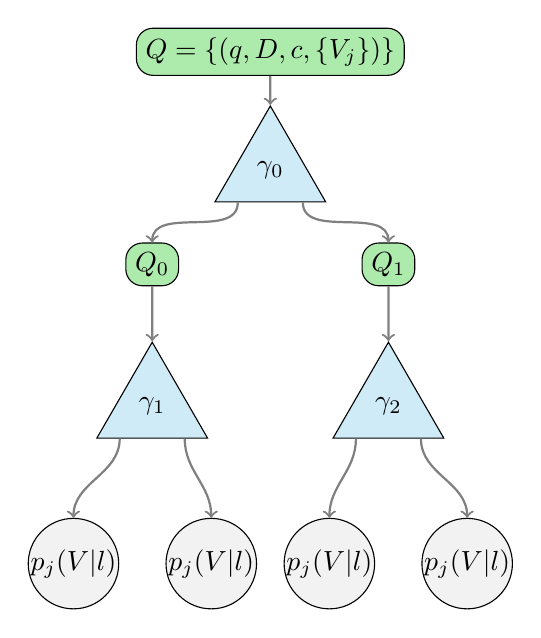
\begin{tikzpicture} [split/.style = {fill=SkyBlue!40, draw, align=center, regular polygon, regular polygon sides=3},
							 leaf/.style = {fill=gray!10, circle, draw, align=center, inner sep=0pt},
							 train/.style = {fill=LimeGreen!40, rectangle, align=center, draw, rounded corners=6pt}]
			\node[train] (t1) at (0, 1.5) {$Q = \{(q,D,c,\{V_j\})\}$};
			\node[split] (s1) at (0, 0) {$\gamma_0$};
			\node[train] (t2) at (-1.5, -1.2) {$Q_0$};
			\node[train] (t3) at (1.5, -1.2) {$Q_1$};
			\node[split] (s2) at (-1.5, -3) {$\gamma_1$};
			\node[split] (s3) at ( 1.5, -3) {$\gamma_2$};
			\node[leaf] (l1) at (-2.5, -5) {$p_j(V|l)$};
			\node[leaf] (l2) at (-0.75, -5) {$p_j(V|l)$};
			\node[leaf] (l3) at ( 0.75, -5) {$p_j(V|l)$};
			\node[leaf] (l4) at ( 2.5, -5) {$p_j(V|l)$};
			
			\draw[->,thick,draw=black!50] (t1.south) to (s1.north) ;
			\draw[->,thick,draw=black!50] (s1.south west) to [out=270,in=90] (t2.north);
			\draw[->,thick,draw=black!50] (s1.south east) to [out=270,in=90] (t3.north);
			\draw[->,thick,draw=black!50] (t2.south) to (s2.north) ;
			\draw[->,thick,draw=black!50] (t3.south) to (s3.north) ;
			\draw[->,thick,draw=black!50] (s2.south west) to [out=270,in=90] (l1.north);
			\draw[->,thick,draw=black!50] (s2.south east) to [out=270,in=90] (l2.north);
			\draw[->,thick,draw=black!50] (s3.south west) to [out=270,in=90] (l3.north);
			\draw[->,thick,draw=black!50] (s3.south east) to [out=270,in=90] (l4.north);
		\end{tikzpicture}	
	\end{figure}

\end{frame}

\begin{frame}
	\frametitle{slitnode}
	\Large
	
	$\Phi_{\textcolor{violet}{\gamma}}(q, D) \mapsto \{0, 1\}$
	
	\vspace{0.5cm}
	
	$\Phi_{\textcolor{violet}{\gamma}}(q, D) = \begin{cases}
	1 & \mbox{if } D(q + \frac{\textcolor{blue}{u}}{D(q)}) - D(q + \frac{\textcolor{blue}{v}}{D(q)}) > \textcolor{blue}{\tau} \\
	0 & \mbox{else}
	\end{cases}$
	
	\vspace{1cm}

	\begin{center}
		\huge
		$\textcolor{violet}{\gamma} = (\textcolor{blue}{u}, \textcolor{blue}{v}, \textcolor{blue}{\tau})$
	\end{center}
	

\end{frame}

\begin{frame}
	\frametitle{choose splitting function}
	\Large

	$\Phi^* = \arg\max_\Phi g(\Phi)$
	\vspace{1cm}
	
	$g(\Phi) = H(Q) - \sum\limits_{s \in \{0, 1\}}^{} \frac{\vert Q_s(\Phi) \vert}{\vert Q \vert} H(Q_s(\Phi))$
	\vspace{1cm}
	
	$H(Q) = - \sum\limits_{c}^{} p(c | Q) \log( p(c | Q) )$
\end{frame}

\begin{frame}
	\frametitle{leafnode}
	\large
	
	A leafnode $l$ stores $p_j(V, l)$
	
	\vspace{0.5cm}
	
	$V_j$ is clustered by mean-shift with Gaussian Kernel with bandwidth $b$
	
	\vspace{0.5cm}
	
	\begin{equation*}
		p_j(V | l) \propto \sum\limits_{k \in K}^{} w_{ljk} \cdot \exp(- \Vert \frac{V - V_{ljk}}{b} \Vert^2_2)
	\end{equation*}
	
	\vspace{0.5cm}
	
	$w_{ljk}$ is determined by offset vectors ended in the cluster k.
\end{frame}

\begin{frame}
	\frametitle{Pose Estimation}
	
	a set of pixels q are sampled in D
	
	\vspace{0.5cm}
	\begin{flalign*}
	 	x_j &= q + V_{ljk} \\
		w_j &= w_ljk \cdot D^2(q) \\
		X_j &= \{(x_j, w_j)\} \\ &&
	\end{flalign*}
	
	\vspace{0.5cm}
	
	\begin{equation*}
		p_j(x | D) \propto \sum\limits_{(x_j, w_j) \in X_j}^{} w_{j} \cdot \exp(- \Vert \frac{x - x_j}{b_j} \Vert^2_2)
	\end{equation*}

	\vspace{0.5cm}
	
	Votes are clustered and only the cluster with the highest summed weights $w_j$ are used for prediction.
\end{frame}

\begin{frame}
	\frametitle{Occlusion Aware Regression Forests}
	
	\begin{flalign*}
		Q_{ext} &= Q \cup Q_{occ} with \\
		Q_{occ} &= \{(q_{occ}, D, c_{occ}, \{v_{jocc}\})\} \\ &&
	\end{flalign*}
	\vspace{0.5cm}
	\begin{equation*}
	p_j(V_{occ} | l) \propto \sum\limits_{k \in K}^{} w_{ljk} \cdot \exp(- \Vert \frac{V_{occ} - V_{ljkocc}}{b} \Vert^2_2)
	\end{equation*}
	\vspace{0.5cm}
	\begin{flalign*}
		X_j &= \{(x_j, w_j)\} \cup \{(x_{jocc}, w_{jocc})\} \\ &&
	\end{flalign*}
\end{frame}

\subsubsection{Trainingsdata}
\begin{frame}
	\frametitle{Training Data}
	\Large
	Synthetic Data (552 images)
	\begin{itemize}
		\item Human Poses from CMU-Database
		\item body part labels for each pixel
	\end{itemize}
	\vspace{1cm}
	Real Data (552 images)
	\begin{itemize}
		\item Kinect2 SDK, all fails are discarded
	\end{itemize}
\end{frame}

\begin{frame}
	\frametitle{Regression Forest}
	\Large
	
	\begin{itemize}
		\item 3 regression trees
		\item max depth = 20
		\item b = 0.05m
	\end{itemize}
	\begin{itemize}
		\item 1000 samples per image
		\item samples 2000 splitting functions per node
	\end{itemize}
\end{frame}

\subsubsection{Results}

\subsection{Occlusion Patterns}
{\setbeamercolor{background canvas}{bg=light-gray}
\begin{frame}
	\frametitle{Occlusion Patterns for Object Class Detection}
	\Large

	\begin{align*}
		\textcolor{blue}{Input}&:  \text{Single RGB-Image} \\
		\textcolor{purple}{Output}&: \text{Object-Boundingboxes}
	\end{align*}
\end{frame}}

\subsubsection{Introduction}
\begin{frame}
	\frametitle{Deformable Models approch}
	\Large
	\begin{itemize}
		\item Consider each object as a deformed version of a template
		\item Compact representation
	\end{itemize}
\end{frame}

\begin{frame}
%	\frametitle{Deformable Models approch}
	\Large
	Matching model to image involves joint optimization of part locations "stretch and fit"
	\vspace{0.5cm}
	\begin{figure}
		\includegraphics[width=8.0cm]{img/pictorialStr.jpeg}
	\end{figure}
\end{frame}

\subsubsection{Algorithm}
\begin{frame}
	\frametitle{Model}
	\large
	Model is represented by a Graph $G = (V, E)$
	\begin{itemize}
		\item $V = p = \{p_0, ..., p_M\}$ are the parts
		\item $p_i$ is parameterized through their bounding box $(l_i, r_i, t_i, b_i)$
		\item $(p_i, p_j) \in E$
	\end{itemize}
	
	\begin{figure}
		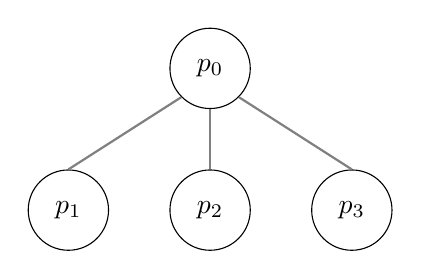
\begin{tikzpicture}[scale=0.9,
							ball/.style = {circle, draw, text width=1cm, align=center, inner sep=0pt}]
			\node[ball] (p0) at (0, 0) {$p_0$};
			\node[ball] (p1) at (-2, -2) {$p_1$};
			\node[ball] (p2) at (0, -2) {$p_2$};
			\node[ball] (p3) at (2, -2) {$p_3$};
			
			\draw[-,thick,draw=black!50] (p0.south west) to (p1.north);
			\draw[-,thick,draw=black!50] (p0.south) to (p2.north);
			\draw[-,thick,draw=black!50] (p0.south east) to (p3.north);
		\end{tikzpicture}
	\end{figure}
	
	\begin{equation*}
		E_c(p; I) = \sum\limits_{i = 0}^{M}\langle v^c_i, \Phi(p_i; I) \rangle + \sum\limits_{i = 1}^{M} \langle w^c_i, \Phi(p_0, p_i) \rangle
	\end{equation*}
	
\end{frame}

\begin{frame}
	\begin{figure}
		\includegraphics[width=\textwidth]{img/trainingDpm.jpg}
	\end{figure}
\end{frame}

\begin{frame}
	\frametitle{OC-DPM}
	\Large
	$C = \{1, ..., C_{visible}\} \cup C_{invisble}$ 
	
	\begin{figure}
		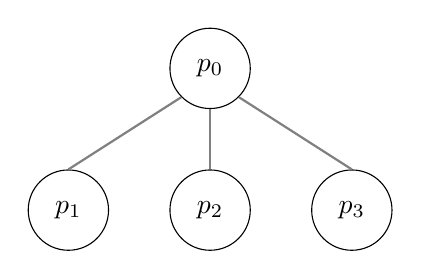
\begin{tikzpicture}[scale=0.9,
							ball/.style = {circle, draw, text width=1cm, align=center, inner sep=0pt}]
			\node[ball] (p0) at (0, 0) {$p_0$};
			\node[ball] (p1) at (-2, -2) {$p_1$};
			\node[ball] (p2) at (0, -2) {$p_2$};
			\node[ball] (p3) at (2, -2) {$p_3$};
			
			\draw[-,thick,draw=black!50] (p0.south west) to (p1.north);
			\draw[-,thick,draw=black!50] (p0.south) to (p2.north);
			\draw[-,thick,draw=black!50] (p0.south east) to (p3.north);
		\end{tikzpicture}
	\end{figure}
\end{frame}

\begin{frame}
	\frametitle{SYM-DPM}
	%\Large
	\begin{align*}
		E'_c(p; I) = \langle v^c_{joint}, \Phi(p_0; I) \rangle 
					&+ \langle \overline{w}, \Phi(\overline{p}_0, p_{joint}) \rangle 
					&&+ \langle \underline{w}, \Phi(\underline{p}_0, p_{joint}) \rangle \\
				    &+ E_c(\overline{p}_0; I) 
				    &&+ E_c(\underline{p}_0; I) \\
	\end{align*}
	
	\begin{figure}
		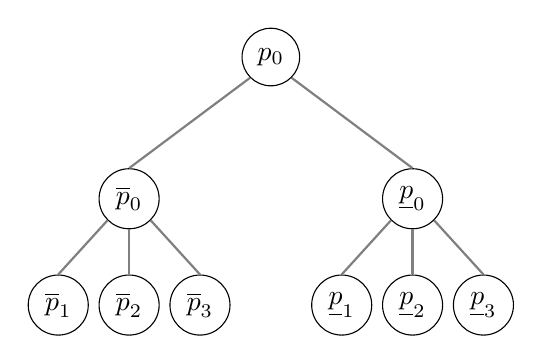
\begin{tikzpicture}[scale=0.9,
							ball/.style = {circle, draw, text width=0.7cm, align=center, inner sep=0pt}]
			\node[ball] (p0) at (0, 0) {$p_0$};
			\node[ball] (p1) at (-2, -2) {$\overline{p}_0$};
			\node[ball] (p2) at (2, -2) {$\underline{p}_0$};
			\node[ball] (p3) at (-3, -3.5) {$\overline{p}_1$};
			\node[ball] (p4) at (-2, -3.5) {$\overline{p}_2$};
			\node[ball] (p5) at (-1, -3.5) {$\overline{p}_3$};
			\node[ball] (p6) at (1, -3.5) {$\underline{p}_1$};
			\node[ball] (p7) at (2, -3.5) {$\underline{p}_2$};
			\node[ball] (p8) at (3, -3.5) {$\underline{p}_3$};
			
			\draw[-,thick,draw=black!50] (p0.south west) to (p1.north);
			\draw[-,thick,draw=black!50] (p0.south east) to (p2.north);
			
			\draw[-,thick,draw=black!50] (p1.south west) to (p3.north);
			\draw[-,thick,draw=black!50] (p1.south) to (p4.north);
			\draw[-,thick,draw=black!50] (p1.south east) to (p5.north);
			
			\draw[-,thick,draw=black!50] (p2.south west) to (p6.north);
			\draw[-,thick,draw=black!50] (p2.south) to (p7.north);
			\draw[-,thick,draw=black!50] (p2.south east) to (p8.north);
		\end{tikzpicture}
	\end{figure}
\end{frame}

\begin{frame}
	\frametitle{ASYM-DPM}	
	\begin{figure}
		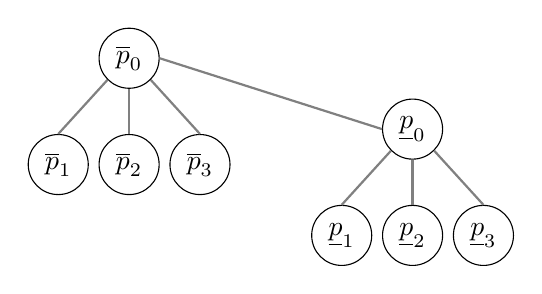
\begin{tikzpicture}[scale=0.9,
							ball/.style = {circle, draw, text width=0.7cm, align=center, inner sep=0pt}]
			\node[ball] (p1) at (-2, 0) {$\overline{p}_0$};
			\node[ball] (p2) at (2, -1) {$\underline{p}_0$};
			\node[ball] (p3) at (-3, -1.5) {$\overline{p}_1$};
			\node[ball] (p4) at (-2, -1.5) {$\overline{p}_2$};
			\node[ball] (p5) at (-1, -1.5) {$\overline{p}_3$};
			\node[ball] (p6) at (1, -2.5) {$\underline{p}_1$};
			\node[ball] (p7) at (2, -2.5) {$\underline{p}_2$};
			\node[ball] (p8) at (3, -2.5) {$\underline{p}_3$};
			
			\draw[-,thick,draw=black!50] (p1.east) to (p2.west);
			
			\draw[-,thick,draw=black!50] (p1.south west) to (p3.north);
			\draw[-,thick,draw=black!50] (p1.south) to (p4.north);
			\draw[-,thick,draw=black!50] (p1.south east) to (p5.north);
			
			\draw[-,thick,draw=black!50] (p2.south west) to (p6.north);
			\draw[-,thick,draw=black!50] (p2.south) to (p7.north);
			\draw[-,thick,draw=black!50] (p2.south east) to (p8.north);
		\end{tikzpicture}
	\end{figure}
\end{frame}

\begin{frame}
	\begin{figure}
	\includegraphics[width=\textwidth]{img/dpmoc_3.png}
	\end{figure}
\end{frame}

\begin{frame}
	\frametitle{KITTI}
	\Large
	\begin{center}
		KITTI contains 7481 images
	\end{center}
	\begin{tabular}{c|c|c|c}
		& $\#$objects & $\#$occluded objects & $\%$ \\
		\hline
		Car & 28521 & 15231 & 53.4 \\
		Pedest. & 4445 & 1805 & 40.6 \\
		Cycles & 1612 & 772 & 44.5 \\
	\end{tabular}
	\vspace{1cm}

	components: 
		\begin{align*}
			\text{\textcolor{blue}{visible} } & 6 \\
			\text{\textcolor{blue}{occluded} } & 16-15 &&\\
		\end{align*}
\end{frame}

\begin{frame}
	\frametitle{Mining Trainingsdata}
	\Large
	Feature Space: \\
	\begin{itemize}
		\item[i]   occluder left/right of occludee
		\item[ii]  orientation of occluder/occludee
		\item[iii] occluder is/is not occluded
		\item[iv] degree of occlusion of occludee
 	\end{itemize}
 	\vspace{1cm}
 	Rule-based clustering
 	\begin{itemize}
	 	\item[] 
 	\end{itemize}
\end{frame}

\subsubsection{Trainingsdata}
\begin{frame}
	\frametitle{Mining Trainingsdata}
	\begin{figure}
	\includegraphics[width=0.7\textwidth]{img/dpmoc_2.png}
	\end{figure}
\end{frame}



\subsubsection{Results}
\begin{frame}
	\begin{figure}
	\includegraphics[width=\textwidth]{img/dpmoc_1.png}
	\end{figure}
\end{frame}

\subsection{Robust Instance Recognition}
{\setbeamercolor{background canvas}{bg=light-gray} 
\begin{frame}
	\frametitle{Robust Instance Recognition in Presence of Occlusion and Clutter}
	\Large
	
	\begin{align*}
		\textcolor{blue}{Input}&:  \text{5-10 consecutive frames as one Pointcloud} \\
		\textcolor{purple}{Output}&: \text{6D-Object-Pose}
	\end{align*}
\end{frame}}
\subsubsection{Introduction}
\begin{frame}
	\frametitle{Overview}
	\begin{figure}
	\includegraphics[width=11cm]{img/rir_2.png}
	\end{figure}
\end{frame}

\subsubsection{Algorithm}
\begin{frame}
	\frametitle{Edgelet}
	
	\begin{columns}
		\begin{column}{0.8\textwidth}
			\begin{itemize}
				\item[] $N$ points per Pointcloud $j$
				\item[] \textcolor{Maroon}{FOR ALL} $i \in \{1, ..., N\}$
						\begin{itemize}
							\item[] calc $\lambda_1$ and $\lambda_2$
							\item[] $r = \frac{\lambda_1}{\lambda_2}$
							\item[] $r \rightarrow$ \textcolor{MidnightBlue}{curvatureMap}
						\end{itemize}
				\item[] hysteresisThesholding(\textcolor{MidnightBlue}{curvatureMap});
				\item[] nonmaximalSuppression(\textcolor{MidnightBlue}{curvatureMap});
				\item[] hysteresisThesholding(\textcolor{MidnightBlue}{depthMap});
				\item[] projectToPointcloud(\textcolor{MidnightBlue}{curvatureMap}, \textcolor{MidnightBlue}{depthMap});
				\item[] RANSAC line fitting
				\item[] orientation to 8 bins\textcolor{OliveGreen}{// (direction$\% \pi$)}
			\end{itemize}
		\end{column}
		\begin{column}{0.2\textwidth}
			\begin{figure}
				
\begin{tikzpicture}[scale=0.7,
									ball/.style = {circle, fill=black!70, text width=0.1cm}]
					\node[ball] (p1) at (-.5, 5) {};
					\draw[->,ultra thick,draw=black!70] (p1.north east) to (.5,6);
				\end{tikzpicture}
			\end{figure}
			\begin{figure}
				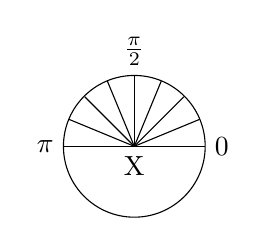
\begin{tikzpicture}[scale=.9]
					\draw (0, 0) ellipse (1 and 1) node[below] {X};
					\draw (-1, 0) node[left]{$\pi$} -- (1, 0)  node[right]{0};
					\draw (0, 0) -- (0, 1)  node[above]{$\frac{\pi}{2}$};
					\draw (0, 0) -- (.7, .7);
					\draw (0, 0) -- (.92, .38);
					\draw (0, 0) -- (.38, .92);
					\draw (0, 0) -- (-.7, .7);
					\draw (0, 0) -- (-.92, .38);
					\draw (0, 0) -- (-.38, .92);
				\end{tikzpicture}
			\end{figure}
		\end{column}
	\end{columns}
\end{frame}

\begin{frame}
	\frametitle{Feature Vector}
	\large
	\begin{columns}
		\begin{column}{.3\textwidth}
			\begin{equation*}
				w \times h \times d
			\end{equation*}
			\begin{figure}
				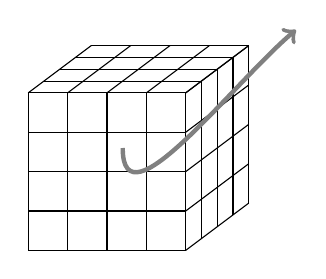
\begin{tikzpicture}[x={(1cm,0cm)},y={(0cm,1cm)}, z={(0.4cm,0.3cm)}, scale=0.5]
					\def\d{2}
					\foreach \x in {-\d, ...,\d} {
						\draw (\x, -\d, -\d) -- (\x, \d, -\d);
						\draw (\x, \d, -\d) -- (\x, \d, \d);
					}
					
					\foreach \y in {-\d, ...,\d} {
						\draw (-\d, \y, -\d) -- (\d, \y, -\d);
						\draw (\d, \y, -\d) -- (\d, \y, \d);
					}
					
					\foreach \z in {-\d, ...,\d} {
						\draw (-\d, \d, \z) -- (\d, \d, \z);
						\draw (\d, -\d, \z) -- (\d, \d, \z);
					}
					\draw[->,ultra thick,draw=black!50] (-.4, 0) to [out=270,in=220] (4, 3);
				\end{tikzpicture}
			\end{figure}
		\end{column}
		\begin{column}{.7\textwidth}
			\begin{center}
				Voxel $v$
			
				\begin{figure}
					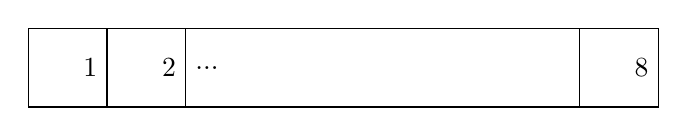
\begin{tikzpicture}
						\draw (0, 0) -- (8, 0) -- node[left]{8}(8, -1) -- (0, -1) -- cycle;
						\draw (1, 0) -- node[left]{1} (1, -1); 
						\draw (2, 0) -- node[left]{2}node[right]{...}(2, -1);
						\draw (7, 0) -- (7, -1);
					\end{tikzpicture}
				\end{figure}
			\end{center}
			\begin{align*}
				x^v_i &= \begin{cases} 1 & \mbox{\textcolor{MidnightBlue}{if} } i \mbox{ is dominant} \\
				0 & \mbox{\textcolor{MidnightBlue}{else} } i \mbox{is not dominant}
				\end{cases} \\
				x^v &= -1 \mbox{ \textcolor{MidnightBlue}{if} v is not visible}
			\end{align*}
		\end{column}
	\end{columns}
	\vspace{1cm}
	The resulting feature vector is the concatenation of all voxels:
	\begin{equation*}
		w \times h \times d \times 8
	\end{equation*}
\end{frame}

\begin{frame}
	\frametitle{Soft Label Random Forest}
	\Large
	\begin{columns}
		\begin{column}{0.5\textwidth}
			\begin{figure}
					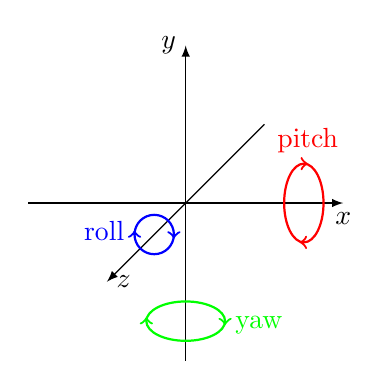
\begin{tikzpicture}[x={(1cm,0cm)},y={(0cm,1cm)}, z={(0.5cm,0.5cm)}, scale=0.5]
						\draw[->, >=latex] (-4,0,0) -- (4,0,0) node[below]{$x$};
						\draw[->, >=latex] (0,-4,0) -- (0,4,0) node[left]{$y$};
						\draw[->, >=latex] (0,0,4) -- (0,0,-4) node[right]{$z$};
						%\draw[semithick, color=green] (,0) arc (270:90:0.5 and 1.5);
						\draw[color=green,thick] (0,-3) ellipse (1 and .5);
						\draw[->,color=green,thick] (-1,-3) -- (-1,-2.9);
						\draw[->,color=green,thick] (1,-3) -- (1,-3.1) node[right]{yaw};
						
						\draw[color=blue,thick] (-.8,-.8) ellipse (.5 and .5);
						\draw[->,color=blue,thick] (-0.3,-.8) -- (-0.3,-.9);
						\draw[->,color=blue,thick] (-1.3,-.8) -- (-1.3,-.7) node[left]{roll};
						
						\draw[color=red,thick] (3,0) ellipse (.5 and 1);
						\draw[->,color=red,thick] (3,1) -- (3.1,1)  node[above]{pitch};
						\draw[->,color=red,thick] (3,-1) -- (2.9,-1);
					\end{tikzpicture}
				\end{figure}
		\end{column}
		\begin{column}{0.5\textwidth}
			\begin{itemize}
				\item 16 pose classes
				\item +1 class $= \begin{cases}
					1 & \mbox{if bg} \\
					0 & \mbox{else}
					\end{cases}$
				\item $d^i_j = \lVert I - R^i_j \rVert_F$
			\end{itemize}
		\end{column}
	\end{columns}
	\begin{align*}
		l^i_j &= \exp ({-d^i_j}^2), i \in \{1, ...,16\} \\
		\text{\textcolor{Maroon}{IF} fg \textcolor{Maroon}{THEN} }1 &= \sum\limits_{i = 1}^{16} l^i_j \text{ \textcolor{Maroon}{ELSE} 0 }
	\end{align*}
\end{frame}

\begin{frame}
\frametitle{}

\begin{figure}
\includegraphics[width=10cm]{img/rir_0.png}
\end{figure}
\end{frame}

\begin{frame}
\frametitle{training scheme for sLRF}

\large

\textcolor{Maroon}{Input}: $X = \{x_j, l_j\}$ \\
\textcolor{Blue}{Output}: Learnt sLRF classifier

\begin{enumerate}
	\item $X_s \subset X$, $\lvert X_s \rvert = \lvert X \rvert / 20$
	\item Train sLRF with $X_s$, compute $p_{fg}$ with X
	\item add borderline positive (low $p_{fg}$) and borderline negativ (high $p_{fg}$)
	\item add confusing samples
	\item compute $d_L$ for all positive samples, add samples with high $d_L$
	\item repeat 2-5 till $p_{fg}$ for all positive data is greater than $p_{fg}$ for all negative data.
\end{enumerate}

\end{frame}

\begin{frame}
	\begin{figure}
	\includegraphics[width=10cm]{img/rir_1.png}
	\end{figure}
\end{frame}



\section{Conclusions}

\begin{frame}
	\frametitle{Conclusion}
	\Large

	\begin{itemize}
		\item redundanze
		\item training with occlusion
		\item semantic (scene understanding)
	\end{itemize}
\end{frame}

\section{Discussion}
{\setbeamercolor{background canvas}{bg=MidnightBlue} \setbeamercolor{titlelike}{fg=white}
\begin{frame}
	\frametitle{Discussion}
	\begin{center}
		{\fontsize{120}{48} \selectfont \textcolor{white}{?}}
	\end{center}
\end{frame}}

\section{References}
\begin{frame}[t,allowframebreaks]
	\nocite{*}
	\printbibliography
\end{frame}

\end{document}
